\documentclass{standalone}
\usepackage{amsmath}
\usepackage{tikz-cd}
\usetikzlibrary{positioning}
\pagecolor{white}
\begin{document}

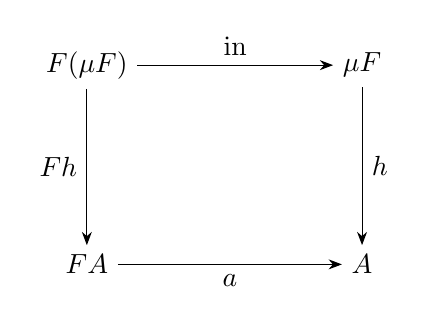
\begin{tikzpicture}[>=Stealth, node distance=2cm]

  \matrix (m1) [matrix of nodes,
                row sep=2cm,
                column sep=2.5cm,
                nodes={anchor=center}] {
    $F(\mu F)$ & $\mu F$ \\
    $F A$      & $A$     \\
  };

  \draw[->] (m1-1-1) -- (m1-2-1) node[midway,left] {$Fh$};
  \draw[->] (m1-2-1) -- (m1-2-2) node[midway,below] {$a$};
  \draw[->] (m1-1-1) -- (m1-1-2) node[midway,above] {in};
  \draw[->] (m1-1-2) -- (m1-2-2) node[midway,right] {$h$};

\end{tikzpicture}
\end{document}
